\chapter{Realisierung}
\section{Einführung}





\section{User Interface}
\subsection{Allgemein}
In diesem Unterabschnitt werden die Konzepte erklärt, mit welchen das User Interface realisiert wurde. Das Webinterface wurde HTML, CSS und JavaScript erstellt und als unterstützende Library wurde Twitter Bootstrap verwendet.

\subsubsection{Java Server Pages JSP}
Sämtlicher HTML Code ist in Java Server Pages (JSP) abgelegt. JSP Seiten werden auf dem Server in Java Servlets kompiliert.
\begin{figure}[H]
\centering
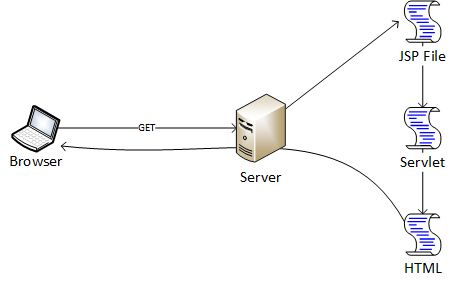
\includegraphics[scale=1]{../04_Realisierung/images/userinterface/jsp.png}
\caption{Java Server Pages}
\end{figure}
Der Client erhält über eine Web-URL vom Server generiertes HTML.

\subsubsection{Java Server Pages Standard Tag Library JSTL}
Mittels JSTL werden in dieser Applikation folgende Aufgaben erfüllt:
\begin{itemize}
\item HTML Fragmente in bestehende Container laden
\item if/else Abfragen für Darstellungen
\item Loop durch Collections im Model für die Darstellung von mehreren Objekten
\end{itemize}

In JSP Seiten wird JSTL mittels folgender Code-Zeile verwendet:
\begin{lstlisting}[language=html5]
<%@ taglib prefix="c" uri="http://java.sun.com/jsp/jstl/core"%>
\end{lstlisting}

Ein Loop durch eine Collection mit Hilfe von JSTP sieht folgendermassen aus:
\begin{lstlisting}[language=html5]
<c:forEach var="collection" items="${collection}">
</c:forEach>
\end{lstlisting}

\subsubsection{Seitenlayout}
Das Seitenlayout ist grundsätzlich sehr einfach. Die Navigation erfolgt am oberen Rand der Seite. Der gesamte Seiteninhalt befindet sich im Content-Bereich. 
\begin{figure}[H]
\centering
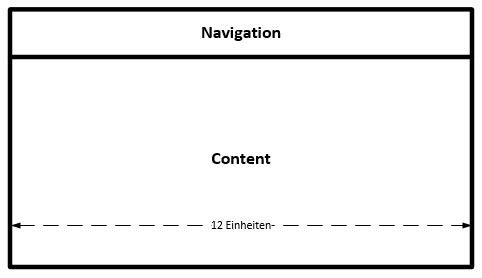
\includegraphics[scale=0.9]{../04_Realisierung/images/userinterface/seitenlayout_allgemein_large.png}
\caption{Seitenlayout Allgemein}
\end{figure}
Das Grid-System von Bootstrap teilt den sichtbaren Bereich in 12 Spalten auf. Jede Spalte besetzt immer $\frac{1}{12}$ der gesamten Fenstergrösse. Bootstrap verwendet folgende CSS Media-Queries für unterschiedliche Bildschirmtypen:
\begin{itemize}
\item Small Devices (min-width: 576px)
\item Tablets (min-width: 768px)
\item Desktops (min-width: 992px)
\item Large Desktops (min-width: 1200px)
\end{itemize}
Sämtlichen div-Containern wird angegeben, wieviele Spalten in welcher Bildschirmgrösse sie besetzen. Mit Bootstrap könnte dies folgendermassen aussehen: 
\begin{lstlisting}[language=html5]
<div class="col-lg-6 col-md-6 col-sm-12 col-xs-12">
</div>
\end{lstlisting}
An diesem Beispiel besetzt dieser Div-Container auf mittelgrossen und grossen Desktops die Hälfte-, auf Tablets und Smartphones die gesamte Bildschirmbreite. Somit wird ein responsives Layout umgesetzt, dass die Applikation sowohl von mobilen-, als auch von Desktop Devices gut nutzbar ist.

\subsubsection{Navigation}
Bootstrap liefert eine ''default-navbar''. Sämtliche Navigationslinks (Home, Device, Discovery, Configurations, User Panel) befinden sich in der Navigationsleiste. Die Navigationsleiste besetzt in jeder Bildschirmgrösse die gesamte Breite.
\begin{lstlisting}[language=html5]
<div class="col-lg-12 col-md-12 col-sm-12 col-xs-12">
</div>
\end{lstlisting}
\begin{figure}[H]
\centering
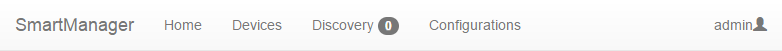
\includegraphics[scale=0.8]{../04_Realisierung/images/userinterface/navbar_lg.png}
\caption{Navigationsleiste gross}
\end{figure}

Da diese Navigationsleiste auf Smartphones schwierig zu bedienen ist, wird auf der kleinsten Bildschirmgrösse anstatt der normalen Links in der Navigation ein Hamburger-Button verwendet. Anfangs war dieser Button stark umstritten, mittlerweile wird er häufig eingesetzt, weshalb jedem Benutzer klar sein sollte, dass sich dahinter weitere Elemente befinden.
\begin{figure}[H]
\centering
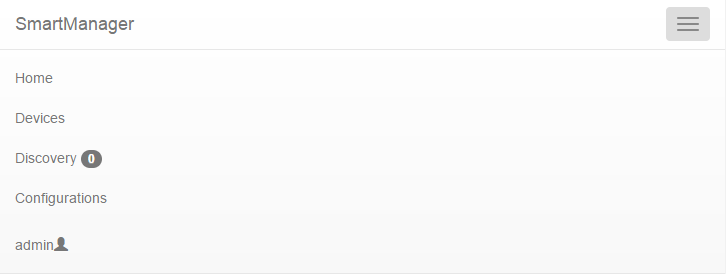
\includegraphics[scale=0.87]{../04_Realisierung/images/userinterface/navbar_xs.png}
\caption{Navigationsleiste xs}
\end{figure}

Die Navigationsleisten sind auf jeder Seite am oberen Bildschirmrand fixiert, sodass bei allfälligem Scrollen die Navigation trotzdem sichtbar bleibt.

Damit duplizierter Code auf jeder Seite verhindert wird, wird der gesamte HTML Code für die Navigation in ein eigenes JSP File ''menuFragment.jsp'' ausgelagert. Der Inhalt des JSP Files wird mittels 
\begin{lstlisting}[language=html5]
<jsp:include page="../../views/menuFragment.jsp" />
\end{lstlisting}
serverseitig ins HTML gerendert.
\subsubsection{Content}
Der gesamte Content Bereich ist auf jeder Seite unterschiedlich gestaltet. Die gesamte Breite von 12 Spalteneinheiten kann verwendet werden.

\subsubsection{Asynchronous JavaScript and XML AJAX}
Damit bei der Kommunikation mit dem Server das User Interface nicht blockiert wird, werden bei sämtlichen Server-Calls AJAX verwendet. AJAX versendet Nachrichten vom Client an den Servern asynchron. Im ''success'' Attribut kann eine Callback-Funktion hinterlegt werden, welche bei erfolgreicher Antwort ausgeführt wird.

In dieser Applikation werden AJAX-Calls nach folgendem Schema ausgeführt:
\begin{lstlisting}[language=js]
$.ajax({
	type : "GET/POST/DELETE",
	url : ctx + "/resource/method",
	success : function() {
		/*some callback code...*/
	},
	error : function(xhr, ajaxOptions, thrownError) {
		window.location.href = ctx + "/";
		alert(thrownError);
	}
});
\end{lstlisting}

Falls der Server mit einem Fehler antwortet, wird die Callback-Funktion im ''error''-Attribut ausgeführt. Der Benutzer wird dabei auf die Haupt-Seite umgeleitet und erhält eine Error-Meldung angezeigt.

\subsubsection{Bootbox}
An verschiedenen Stellen auf der Seite werden Pop-ups benötigt. In diesem Projekt wird die JavaScript Library ''Bootbox'' von Bootboxjs.com verwendet.

\begin{figure}[H]
\centering
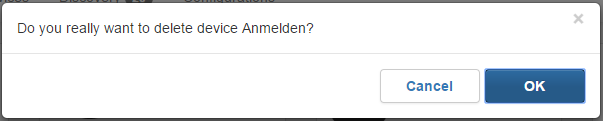
\includegraphics[scale=0.9]{../04_Realisierung/images/userinterface/bootbox.png}
\caption{Bootbox}
\end{figure}

Der JavaScript Code für die Erstellung und Verwendung der Bootbox ist leicht verständlich.

\begin{lstlisting}[language=js]
bootbox.confirm({
	size : "large",
	title : "some title",
	message : content,
	callback : function(ok) {
		if (ok) {
			/*save, redirect etc.*/		
		}
	}
});
\end{lstlisting} 

Als ''message''-Attribut kann ein String oder auch HTML Code eingefügt werden.  Beim ''Callback''-Attribut kann eine Callback-Funktion hinterlegt werden. Diese wird ausgeführt, wenn das Pop-up Fenster geschlossen wird. Die if-Abfrage stellt sicher, dass der darinliegende Code nur ausgeführt wird, wenn ''OK'' auf geklickt wird.

\subsubsection{Google Maps API}
An verschiedenen Stellen auf der Seite werden Devices auf Google Maps Karten angezeigt. Dies gibt dem Benutzer eine schnelle Übersicht der Lokalitäten der IoT Devices.

Über die JavaScript-Funktion ''initMap()'' wird die (leere) Map geladen. Danach werden über die Funktion ''getLocations()'' die Locations der benötigten IoT Devices vom Server abgefragt. Über die ''insertLocations()''-Funktion werden die Punkte auf der Map eingezeichnet.

\subsection{Home}
Die Home-Seite dient als Einstiegspunkt und Übersichtsseite. Dem Benutzer sollen Informationen über die Applikation und die verwaltete Infrastruktur angezeigt werden.

\begin{figure}[H]
\centering
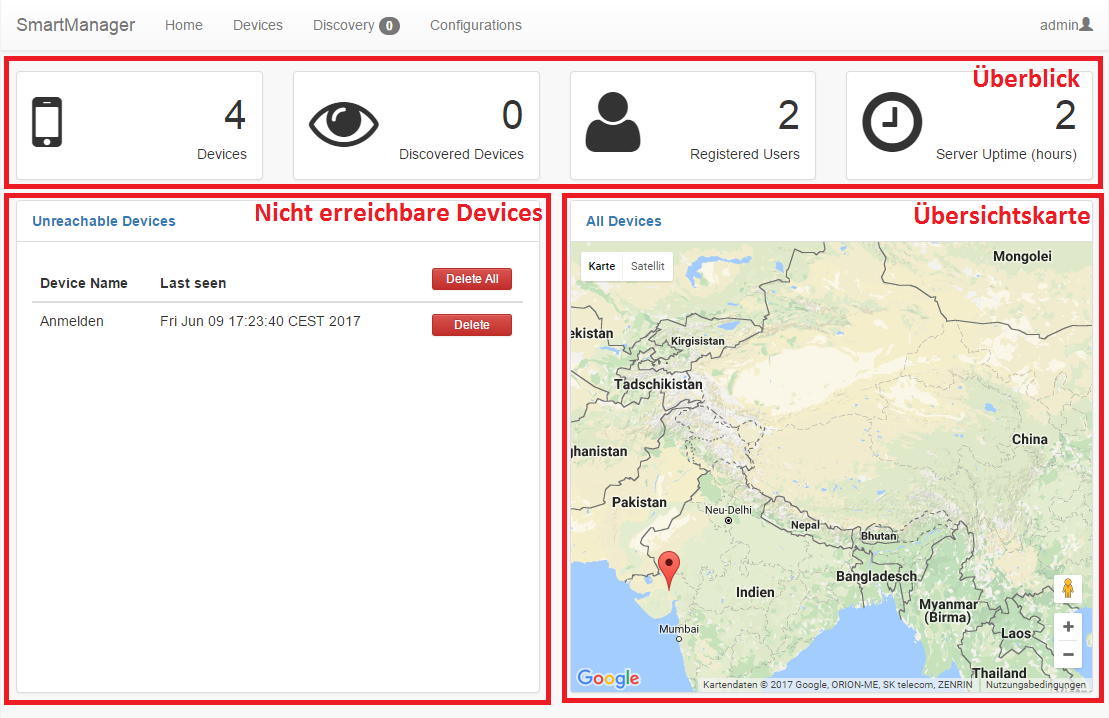
\includegraphics[scale=0.57]{../04_Realisierung/images/userinterface/home.png}
\caption{Dashboard}
\end{figure}

\subsubsection{Überblick}
In diesem Bereich werden dem Benutzer folgende vier Informationen auf den ersten Blick angezeigt:
\begin{itemize}
\item Gesamtanzahl erfasster Devices im System
\item Anzahl Devices im Discovery (noch nicht verwaltet)
\item Anzahl registrierter Benutzer
\item Server Uptime in Stunden
\end{itemize}

\subsubsection{Nicht erreichbare Devices}
Sind Devices nicht mehr erreichbar, muss dies dem Benutzer mitgeteilt werden. Hat sich ein Device mehr als 30 Minuten nicht mehr beim Server gemeldet, so erscheint es in dieser Tabelle. Klickt der Benutzer auf ''Delete'' respektive ''Delete All'', so werden die JavaScript Funktionen ''deleteUnreachableDevice(id, name)'' und ''deleteAllUnreachableDevices()'' ausgeführt. Über eine AJAX-Anfrage werden die entsprechenden Serverpfade aufgerufen.

\subsubsection{Übersichtskarte}
Auf dieser Übersichtskarte werden alle im Device gespeicherten Locations von IoT Devices angezeigt.

\newpage
\subsection{Discovery}
Auf der Discovery Seite sieht der Benutzer alle registrierten Devices. Sämtliche Devices registrieren sich am LwM2M Server. Sind sie vom Benutzer noch nicht hinzugefügt worden, so erscheinen sie auf dieser Seite.

\begin{figure}[H]
\centering
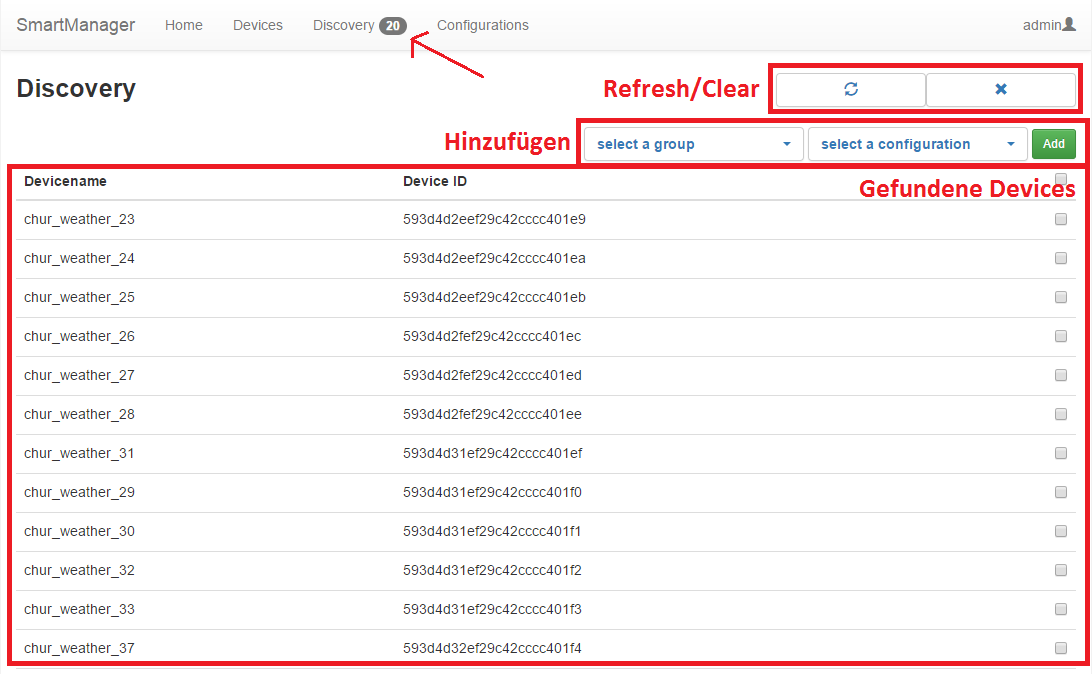
\includegraphics[scale=0.57]{../04_Realisierung/images/userinterface/discovery.png}
\caption{Discovery}
\end{figure}

\subsubsection{Gefundene Devices}
Ist ein Device vom Benutzer noch nicht hinzugefügt worden, besitzt das Attribut ''added'' den Wert ''false''. Nachdem der Benutzer das Device hinzugefügt hat, wird dem Device das Attribut ''added'' auf ''true'' gesetzt und erscheint deshalb nicht mehr.

\subsubsection{Hinzufügen}
Beim ''Add''-Button werden die selektierten Devices hinzugefügt. Es besteht die Möglichkeit, beim Hinzufügen eine Gruppe oder eine Initiale Konfiguration zu setzen.

\begin{figure}[H]
\centering
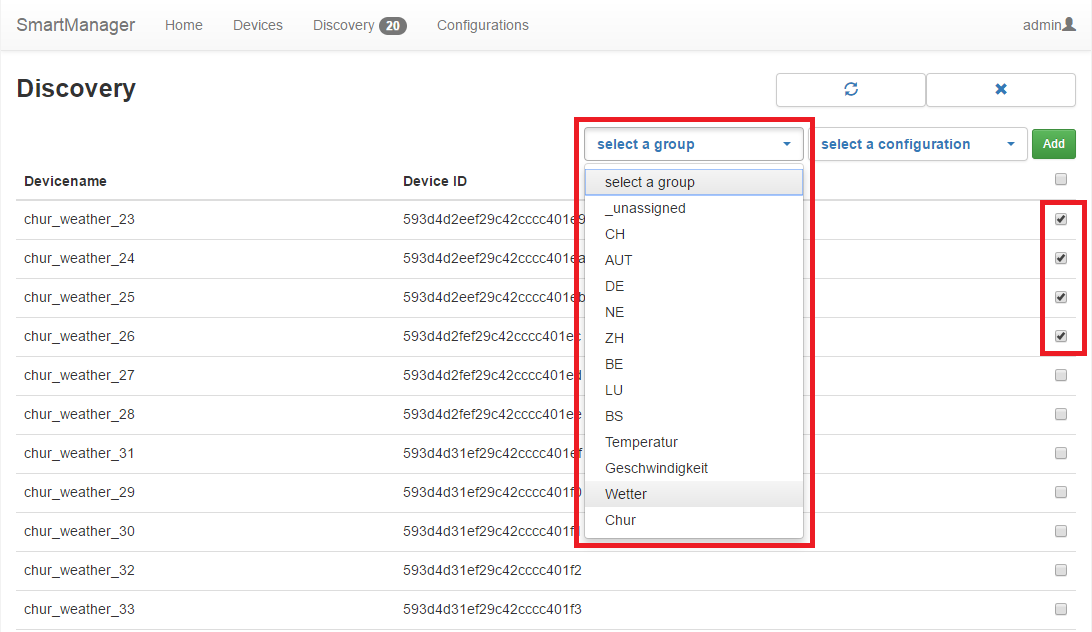
\includegraphics[scale=0.57]{../04_Realisierung/images/userinterface/discovery_addgroup.png}
\caption{Discovery Gruppenauswahl}
\end{figure}

Die selektierten Werte in den Drop-Down-Listen werden dem Server beim Hinzufügen des Devices übergeben.

\subsubsection{Refresh/Clear}
Mit dem Refresh Button wird die Seite neu geladen, damit frisch registrierte Devices angezeigt werden. Der Clear Button leert die Liste von Devices. Melden sich die Devices zu einem späteren Zeitpunkt nochmals, so tauchen sie in dieser Ansicht wieder auf.

\subsection{Configuration}
Benutzer können auf dieser Seite eigene Konfigurationen erstellen. Sämtliche schreibbaren LwM2M-Objekte können gesetzt werden. Nach der Erstellung einer Konfiguration kann sie auf neue Devices oder eine Devicegruppe geschrieben werden.

\begin{figure}[H]
\centering
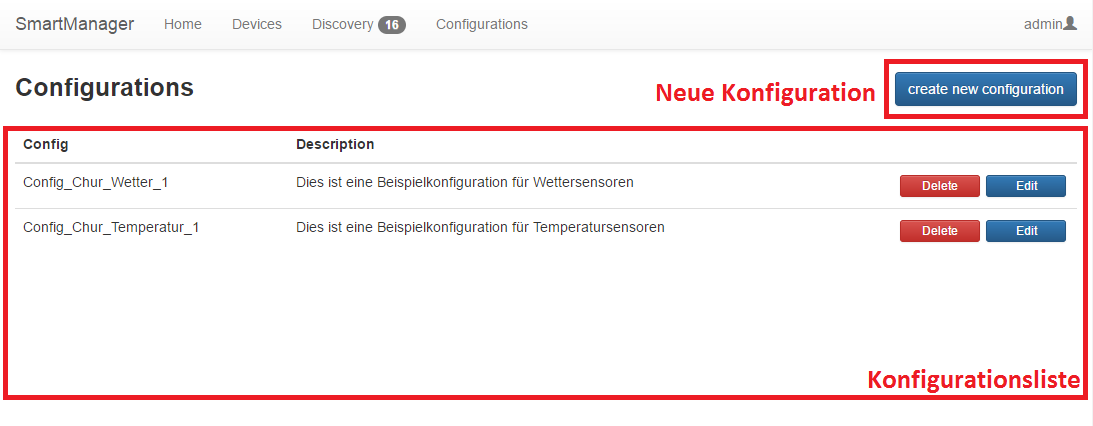
\includegraphics[scale=0.57]{../04_Realisierung/images/userinterface/config_overview.png}
\caption{Configuration Übersicht}
\end{figure}

\subsubsection{Konfigurationslisten}
Sämtliche erstellten Konfigurationen werden hier aufgelistet. Eine Konfiguration kann einzeln gelöscht und editiert werden.

\subsubsection{Neue Konfiguration}
Mit dem ''create new configuration'' Button öffnet sich ein neues Pop-up, in welchem der Benutzer eine neue Konfiguration erstellt.

\begin{figure}[H]
\centering
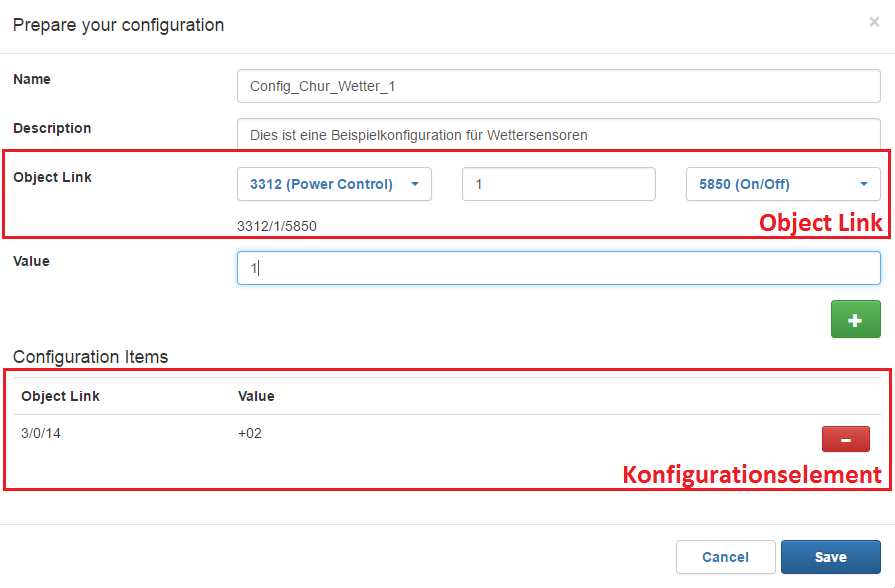
\includegraphics[scale=0.7]{../04_Realisierung/images/userinterface/config.png}
\caption{Configuration Neu}
\end{figure}

Sowohl Name, als auch Description können frei gewählt werden. Beim selektieren der Object ID (linkes Drop-Down Menü) wird eine Ajax Anfrage an den Server gesendet. Als Antwort erhält man informationen über die beiden anderen Felder. Sind Multi-Instanzen nicht erlaubt, so bleibt das Zahlenfeld ausgegraut, die Daten für das rechte Drop-Down werden dynamisch gerendert, sind also abhängig von der links gewählten Object-ID. Das Value Feld kann frei beschrieben werden. Serverseitig werden Überprüfungen des Typs, sowie Character Escaping durchgeführt.

Nachdem der Benutzer den Plus-Button geklickt hat, erscheinen Object Link und Value als Configuration Item in einer Liste und es kann mit weiteren Einstellungen forgefahren werden. Sobald der Benutzer ''Save'' drückt, wird clientseitig ein JSON-formatiertes Konfigurationsobject erstellt und an den Server gesendet.

\begin{lstlisting}[language=json]
[
  "Config_Chur_Temperatur_1", 
  "Dies ist eine Beispielkonfiguration fuer Temperatursensoren", 
  {
	"Object Link": "3305/0/5806",
	"Value": "5.5382"
  }, 
  {
	"Object Link": "3201/0/5750",
	"Value": "I/O"
  }
]
\end{lstlisting}



\subsection{Devices und Groups}
Benutzer können auf dieser Seite einzelne Devices und Gruppen verwalten. Sie ist also sozusagen das Kernstück der Applikation, da viele Use-Cases in diesem Bereich abgedeckt werden.

\begin{figure}[H]
\centering
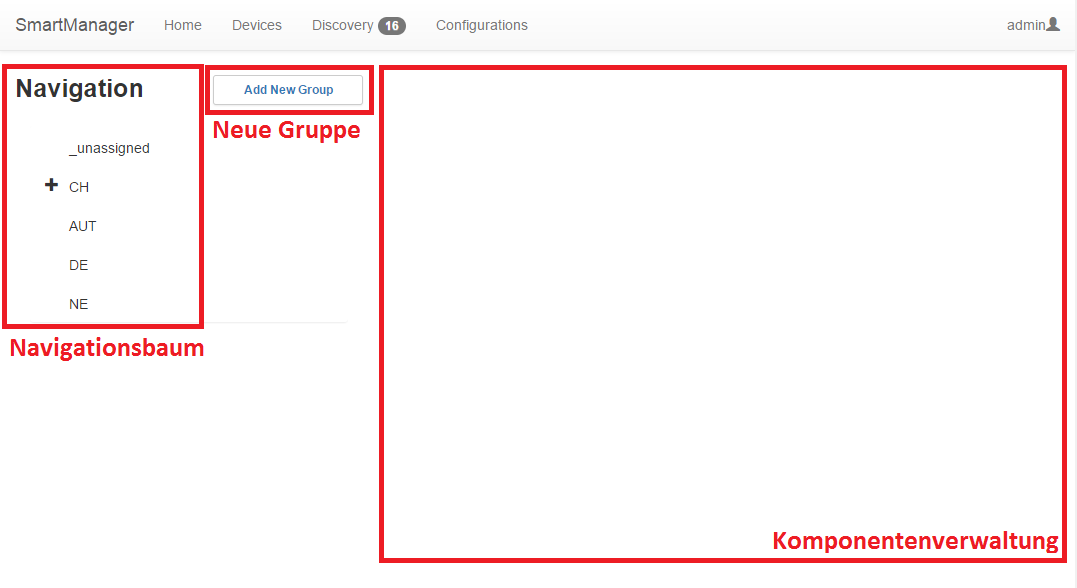
\includegraphics[scale=0.57]{../04_Realisierung/images/userinterface/devices_start.png}
\caption{Devices}
\end{figure}

\subsubsection{Komponentenverwaltung}
Der Bereich der Komponentenverwaltung ist zu Beginn leer. Der Benutzer muss zuerst eine Gruppe oder ein Device selektieren, damit der entsprechende Inhalt geladen wird. Es gibt zwei verschiedene Komponentenverwaltungen, die Device- und die Gruppenverwaltung. Nachdem im Navigationsbereich link eine Gruppe/Device gewählt wurde, wird vom Server ein HTML Fragment angefordert und dargestellt.

\subsubsection{Navigationsbaum}
Auf der linken Seite befindet sich der Navigationsbaum. Darin befinden sich sämtliche Gruppen und Devices hierarchisch angeordnet. 

\begin{figure}[H]
\centering
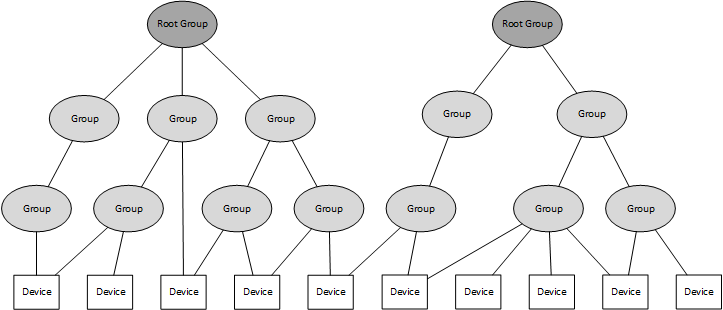
\includegraphics[scale=0.84]{../04_Realisierung/images/userinterface/componentstree.png}
\caption{Komponentenbaum}
\end{figure}

Gruppen dürfen beliebig tief verschachtelt werden, sind jedoch einzigartig und haben höchstens eine direkte Elterngruppe. Es dürfen beliebig viele Root Gruppen bestehen. Diese erscheinen in der Navigation zuoberst (ohne aufklappen zu müssen), ansosten unterscheiden sie sich nicht von ''normalen'' Gruppen. 

Devices entsprechen den Blattknoten, sie dürfen keine Kindsknoten enthalten. Devices dürfen aber bei beliebig vielen Gruppen als Kindsknoten existieren, somit hat der Benutzer maximale Freiheiten beim Verwalten seiner Devices.

Der Navigationsbaum wurde mit Hilfe der gijgo Library implementiert. Gijgo ist eine JavaScript (jQuery) Library, welche aus Baumstrukturen aufklappbare Navigationen erstellt.

\begin{lstlisting}[language=js]
$('#tree').tree(
	{
		primaryKey : 'id',
		uiLibrary : 'bootstrap',
		dataSource : ctx + '/groups/getAll'
	});
\end{lstlisting}

Die Verwendung der Library ist sehr simpel. Auf einem selektierten Div-Container kann die Funktion tree() ausgeführt werden. Als Datenquelle wird eine URL angegeben. Diese API liefert die Baumstruktur im JSON Format, welche von der Gijgo-Library direkt interpretiert wird.

Anbei ist ein einfaches Beispiel einer Komponentenhierarchie.

\begin{lstlisting}[language=json]
[
	{
		"id": "groups/593e584eed204e174c2a0cc4",
		"text": "ZH",
		"children": 
	  	[
		  	{
				"id": "devices/593e5845ed204e174c2a0cae",
				"text": "chur_weather_23"
			},
			{
				"id": "devices/593e5845ed204e174c2a0caf",
				"text": "chur_weather_24"
			}
		]
	}
]
\end{lstlisting}

\subsection{Devices}
Wählt man in der Navigation ein Device an, so wird eine Anfrage für das HTML Fragment für Devices gestartet. 

\begin{figure}[H]
\centering
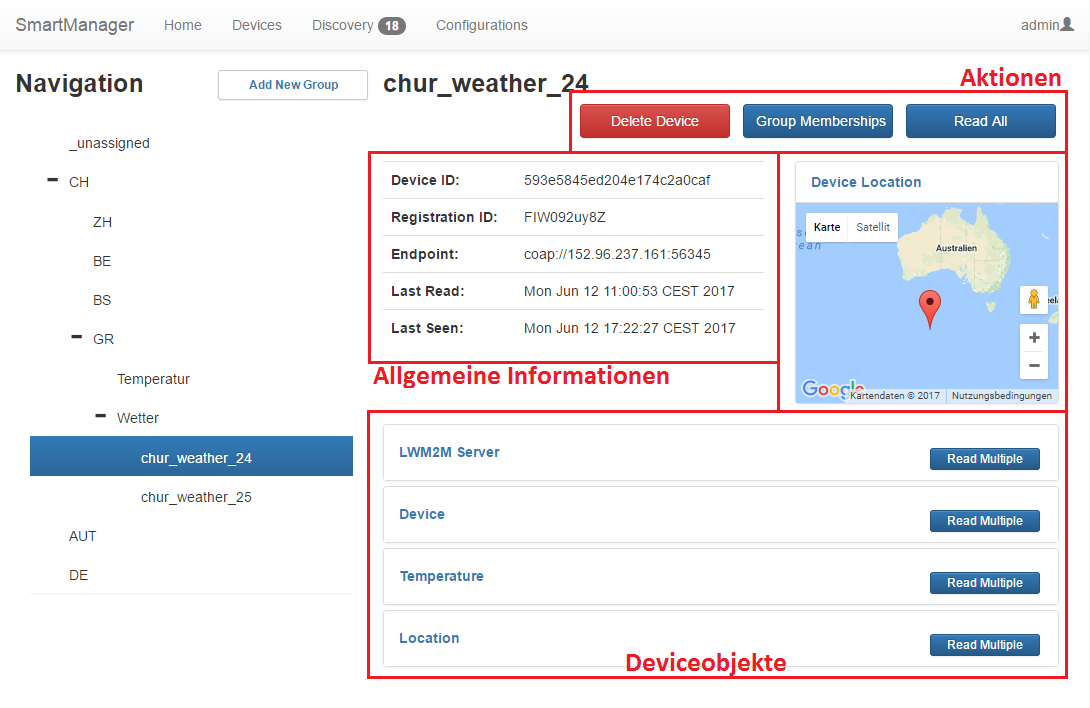
\includegraphics[scale=0.57]{../04_Realisierung/images/userinterface/devicefragment_collapsed.png}
\caption{Übersicht einzelnes Device}
\end{figure}

\subsubsection{Aktionen}
Mit ''Delete Device'' wird das Device komplett von der Datenbank entfernt. Mit ''Group Memberships'' kann das Device unterschiedlichen Gruppen zugewiesen werden. ''Read All'' führt ein Lesevorgang über sämtliche verfügbaren Objekte (siehe weiter unten).

\subsubsection{Allgemeine Informationen}
Im Bereich der allgemeinen Informationen erhält der Benutzer nützliche Device-Details angezeigt, ebenfalls wird mittels Google Maps API die Location des Devices automatisch angezeigt.

\subsubsection{Deviceobjekte}
Die Deviceobjekte sind standardmässig zugeklappt. Die einzelnen Objekte sind jeweils eine aufklappbare Panels. Bei der Registration meldet ein Device dem LwM2M Server, welche Objekte es unterstützt. Die Panels werden, abhängig der unterstützten Objekte, dynamisch erzeugt. Mit dem ''Read Multiple'' Button werden sämtliche Felder des Objekts gelesen.

\begin{figure}[H]
\centering
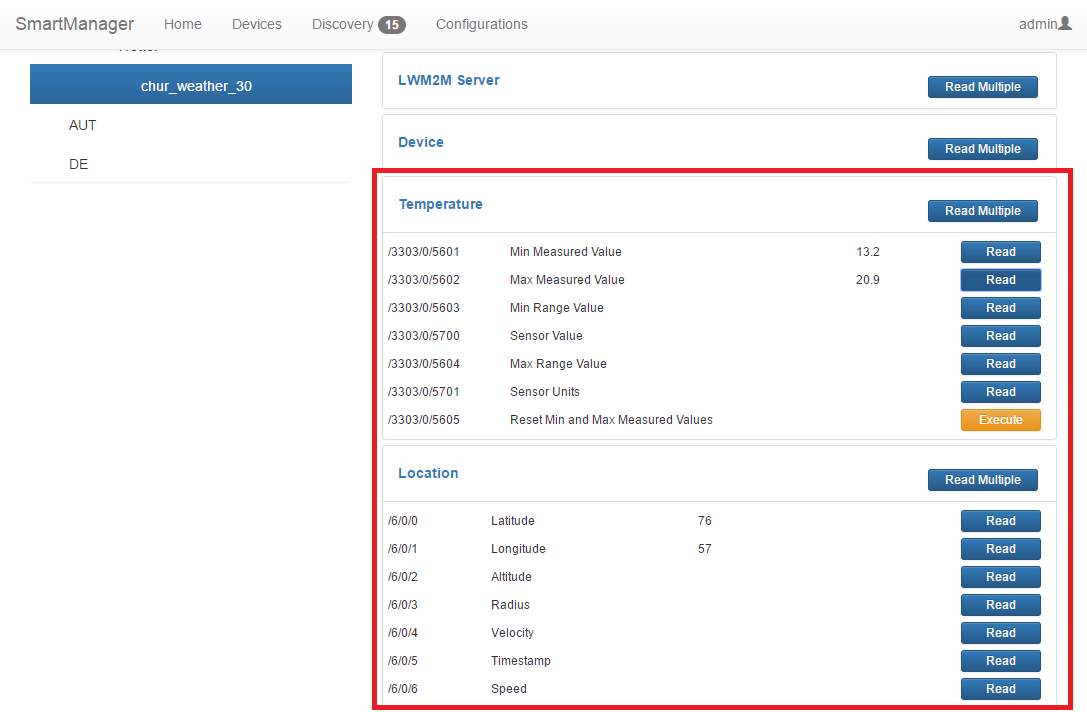
\includegraphics[scale=0.57]{../04_Realisierung/images/userinterface/devicefragment.png}
\caption{Anzeige Objektdetails}
\end{figure}

Sobald der Benutzer ein Panel anklickt, werden die darunterliegenden Attribute in einer dynamisch generierten Tabelle angezeigt. Zu Beginn sind noch keine Werte vorhanden. Es muss entweder pro Feld einzeln-, oder über den ''Read Multile''- respektive ''Read All''-Button vom Device gelesen werden.

Auf der rechten Seite werden Buttons für die unterstützen Aktionen angezeigt. Jede Instance ID hat in der XML-Spezifikation hinterlegt, welche Aktionen verfügbar sind.

\begin{figure}[H]
\centering
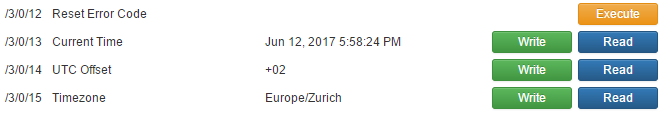
\includegraphics[scale=0.7]{../04_Realisierung/images/userinterface/rwe.png}
\caption{RWE Buttons}
\end{figure}

\subsection{Groups}
In der Gruppenansicht stehen dem Benutzer viele Funktionen für die Verwaltung von Devices und Groups zur Verfügung. In der Map-Übersicht sind alle Devices ersichtlich.

\subsubsection{Group Members}
Gruppenmitglieder können unter ''Group Members'' verwaltet werden. 

\begin{figure}[H]
\centering
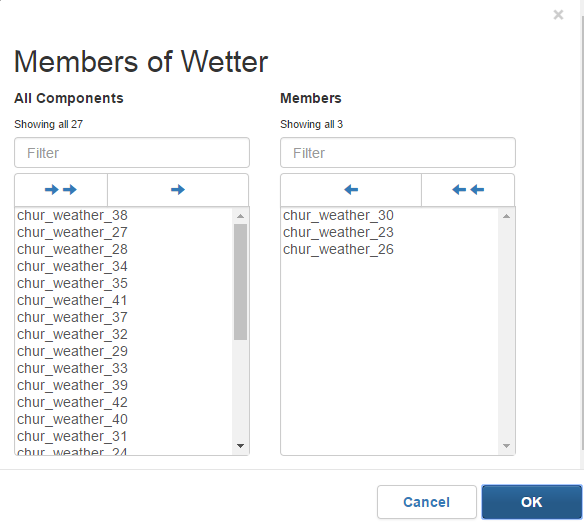
\includegraphics[scale=0.8]{../04_Realisierung/images/userinterface/groupmembers.png}
\caption{Gruppenmitglieder}
\end{figure}

Sowohl Devices, als auch Gruppen werden auf der linken Seite angezeigt, diese können hinzugefügt werden. Die Liste wird mittels Ajax-Anfrage vom Server abgerufen. Es wird ein Delta zwischen der Menge aller Komponenten und den aktuellen Mitgliedern erstellt.

Auf der rechten Seite sind die Mitglieder aufgelistet, sobald ''OK'' gedrückt wird, wird eine Liste mit den angepassten Mitgliedern an den Server gesendet.

Diese Verwaltung wurde mit Hilfe der Bootstrap-Duallist-Box Library implementiert. 
\subsubsection{Group Memberships}
Die Mitgliedschaft 

\subsubsection{Add New Child Group}

\subsubsection{Write Configuration}

\subsubsection{Execute}

\subsubsection{Write}

\begin{figure}[H]
\centering
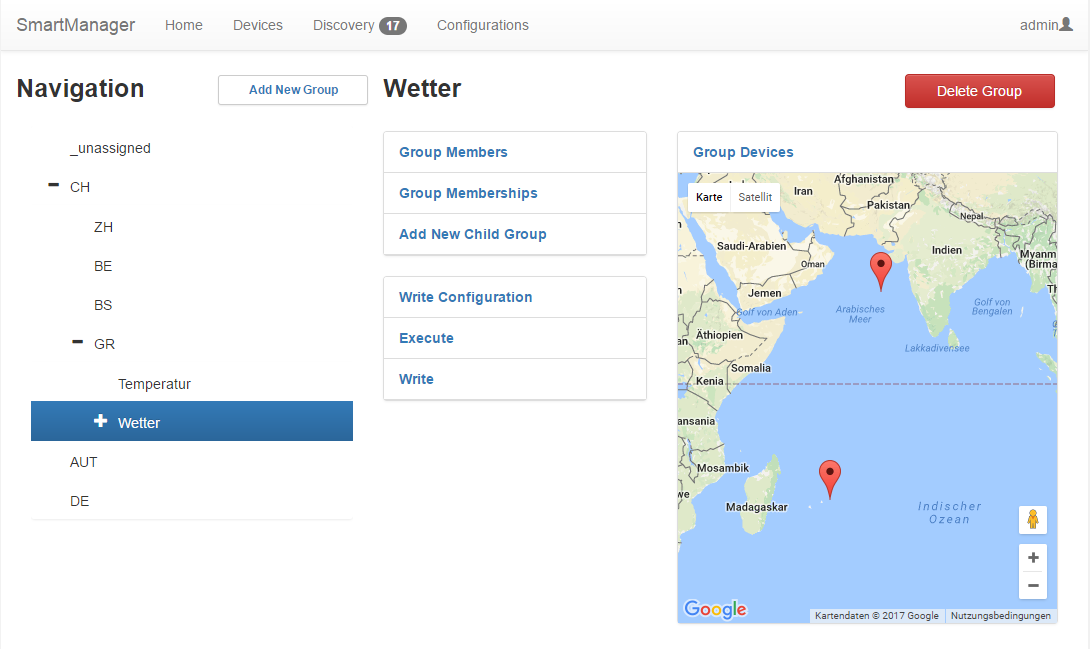
\includegraphics[scale=0.57]{../04_Realisierung/images/userinterface/groups.png}
\caption{Gruppenansicht}
\end{figure}



\newpage

\section{Controllers}
\subsection{Allgemein}
Mit dem Controller-Layer werden alle Routen und Web API Methoden definiert. Für dies wurde das Spring Framework mit der spring-webmvc (v4.3.7) und der spring-web (v4.3.7) Library verwendet. Das Spring Framework hat dabei viel Arbeit abgenommen und den grossen Teil bereits implementiert. Im Controller wurden daher nur noch die Daten aus dem Service-Layer geholt, mit der View verbunden und an den Client zurückgesendet.

\subsection{Verwendete Annotations}
\subsubsection{@Controller}
Die @Controller Annotation ist die Spring Bezeichnung für einen Web Controller. Diese Annotation wird direkt über dem Klassennamen platziert. Hier sieht man das Beispiel des DeviceWebController:
\begin{lstlisting}[language=java]
@Controller
@RequestMapping("/devices")
public class DeviceWebController {
...
}
\end{lstlisting}

Der Controller führt die zur Route passende Methoden aus, holt die Daten aus dem Service Layer und mappt diese auf das Model und gibt die View mit den Daten zurück. Dabei ist der Rückgabe immer der Name der View und wird als String an das Spring Framework übergeben.

Dies ist ein Beispiel von der /groups/id Route. Als ersten Schritt wird die Gruppe aus dem Service-Layer geholt und dem Model hinzugefügt. Danach gibt man im Return-Wert die gewünschte View-Datei an. Hier im Beispiel ist dies die groupFragment.jsp Datei. Der ganze Rest wird durch Spring und der Template Engine erledigt.
\begin{lstlisting}[language=java]
@RequestMapping(value = "/{id}", method = RequestMethod.GET)
public String showGroupDetails(Model model, @PathVariable("id") String id) {
	model.addAttribute("group", groupService.getGroup(id));
	return "devices/groupFragment";
}
\end{lstlisting}
\subsubsection{@RestController}
Die zweite Controllerart ist der RestController. Auch diese Annotation wird direkt oberhalb des Klassennamens platziert. Im gegensatz zur @Controller Annotation gibt der RestController Daten im JSON-Format zurück. 

Die Rückgabewerte werden von Spring automatisch in das JSON-Format umgewandelt und an den Client gesendet. Dies setzt voraus, dass der Rückgabetyp entweder eine get-Methode auf alle Felder besitzt oder ein einfacher Datentyp wie zum Beispiel String ist.
Hier sieht man, wie eine Restmethode aussehen könnte. Es werden alle Gruppen aus dem Service-Layer geholt und als JSON an den Client gesendet.
\begin{lstlisting}[language=java]
@RequestMapping(value = "/list", method = RequestMethod.GET)
public List<DeviceGroup> getGroupList() {
	return groupService.getAllGroups();
}
\end{lstlisting}

Das durch Spring generierte JSON sieht wie folgt aus:
\begin{lstlisting}[language=json]
[
    {
        "id": "593e57293f56e959e84339f9",
        "name": "_unassigned",
        "children": []
    },
    {
        "id": "593e828a3f56e96a8b665fa8",
        "name": "CH",
        "children": [
            {
                "id": "593e82903f56e96a8b665fa9",
                "name": "Luzern",
                "children": []
            }
        ]
    },
    {
        "id": "593e82903f56e96a8b665fa9",
        "name": "Luzern",
        "children": []
    }
]
\end{lstlisting}

\subsubsection{@RequestMapping}
Durch das RequestMapping gibt man die Route und die Methode an, auf welche der Controller reagieren soll. Diese Annotation kann bei der Klasse, sowie bei jeder Methode angegeben werden. Gibt man das RequestMapping bei der Klasse an, gilt dieses für alle weiteren Methoden in der Klasse.

Hier sieht man wie die Route /users/delete mit der Requestmethode POST definiert wird. Durch diese zwei Annotationen weiss Spring, dass diese Methode ausgeführt werden muss.
\begin{lstlisting}[language=java]
@RestController
@RequestMapping("/users")
public class UserRestController {

	@RequestMapping(value = "/delete", method = RequestMethod.POST)
	public String deleteUser(@RequestParam("username") String username) {}
	...
}
\end{lstlisting}
\subsubsection{@PathVariable}
Um einer Route eine Pfadvariable zu hinterlegen, gibt es die PathVariable Annotation. Diese wird in der Parameterliste der Methode eingefügt, um die Werte aus der Route zu erhalten.

In diesem Beispiel wurde eine Pfadvariable Id definiert. Dies geschieht durch die geschweiften Klammern. Um die Variable in der Methode benutzen zu können, wird die @PathVariable eingefügt. Dadurch nimmt Spring den Id-Teil der Route und wandelt es in diesem Beispiel zu einem String um. So kann man die Variable in der gesamtem Methode verwenden.
\begin{lstlisting}[language=java]
@RequestMapping(value = "/{id}/delete", method = RequestMethod.DELETE)
public void removeGroup(@PathVariable("id") String id) {
	groupService.deleteGroup(id);
}
\end{lstlisting}
\subsubsection{@RequestParam}
Um Request Parameter abzufangen, gibt es die @RequestParam Annotation. Durch diese können zum Beispiel Formulardaten abgefangen werden und der Methode zur Verfügung gestellt werden. Dazu werden alle zu erwarteten Request Parameter als Variable in der Parameterliste der Methode an.

In diesem Beispiel wird eine List von Strings übergeben. Der Post muss den Parameter auch value nennen, damit Spring dies richtig erkennt. Wird alles korrekt übergeben, wandelt Spring die erhaltenen JSON-Daten in das gewünschte Format um.
\begin{lstlisting}[language=java]
@RequestMapping(value = "/{id}/removeFromGroups", method = RequestMethod.POST)
public void removeFromGroups(@PathVariable("id") String id, @RequestParam("value") List<String> value) {
	groupService.removeDeviceFromGroups(value, id);
}
\end{lstlisting}
\subsection{Übersicht aller Routen}
\begin{longtable}{ p{11cm} p{4cm} l}
\hline 
\multicolumn{1}{p{11cm}}{\textbf{URI}} & 
\multicolumn{1}{p{4cm}}{\textbf{Method}} &  \\ \hline 
\endfirsthead

\hline 
\multicolumn{1}{p{11cm}}{\textbf{URI}} & 
\multicolumn{1}{p{4cm}}{\textbf{Method}} &  \\ \hline 
\endhead

/	&	GET	 \\ \addlinespace
/login	&	GET	 \\ \addlinespace
/logout	&	GET	 \\ \addlinespace
/users	&	POST	 \\ \addlinespace
/users/add	&	POST	 \\ \addlinespace
/users/delete	&	POST	 \\ \addlinespace
/users/checkUser	&	POST	 \\ \addlinespace
/users/userAddFragment	&	GET	 \\ \addlinespace
/users/userDeleteFragment	&	GET	 \\ \addlinespace
/users/userEditFragment	&	GET	 \\ \addlinespace
/users/{id}/edit	&	POST	 \\ \addlinespace
/discovery	&	GET	 \\ \addlinespace
/discovery/clean	&	GET	 \\ \addlinespace
/configurations	&	GET	 \\ \addlinespace
/configurations/add	&	POST	 \\ \addlinespace
/configurations/createConfigurationFragment	&	GET	 \\ \addlinespace
/configurations/delete	&	POST	 \\ \addlinespace
/configurations/{id}/editConfigurationFragment	&	GET	 \\ \addlinespace
/devices	&	GET	 \\ \addlinespace
/devices/add	&	POST	 \\ \addlinespace
/devices/deleteAll	&	DELETE	 \\ \addlinespace
/devices/locations/dashboard	&	GET	 \\ \addlinespace
/devices/{id}	&	GET	 \\ \addlinespace
/devices/{id}/changeMembership	&	POST	 \\ \addlinespace
/devices/{id}/delete	&	DELETE	 \\ \addlinespace
/devices/{id}/memberships	&	GET	 \\ \addlinespace
/devices/{id}/removeFromGroups	&	POST	 \\ \addlinespace
/devices/{id}/locations/{mapType}	&	GET	 \\ \addlinespace
/devices/{id}/read/{objectId}	&	GET	 \\ \addlinespace
/devices/{id}/execute/{objectId}/{objectInstanceId}/{resourceId}	&	GET	 \\ \addlinespace
/devices/{id}/write/{objectId}/{objectInstanceId}/{resourceId}	&	POST	 \\ \addlinespace
/devices/{id}/read/{objectId}/{objectInstanceId}/{resourceId}	&	GET	 \\ \addlinespace
/groups/add	&	POST	 \\ \addlinespace
/groups/getAll	&	GET	 \\ \addlinespace
/groups/list	&	GET	 \\ \addlinespace
/groups/executeCommandToChildsFragment	&	GET	 \\ \addlinespace
/groups/writeCommandToChildsFragment	&	GET	 \\ \addlinespace
/groups/writeConfigToChildsFragment	&	GET	 \\ \addlinespace
/groups/{id}	&	GET	 \\ \addlinespace
/groups/{id}/add	&	POST	 \\ \addlinespace
/groups/{id}/changeMembers	&	POST	 \\ \addlinespace
/groups/{id}/changeMembership	&	POST	 \\ \addlinespace
/groups/{id}/delete	&	DELETE	 \\ \addlinespace
/groups/{id}/members	&	GET	 \\ \addlinespace
/groups/{id}/memberships	&	GET	 \\ \addlinespace
/groups/{id}/writeChildDevices/{objectId}/{objectInstanceId}/{resourceId}	&	GET	 \\ \addlinespace
/groups/{objectId}/executeToChildren	&	GET	 \\ \addlinespace
/groups/{objectId}/multiInstance	&	GET	 \\ \addlinespace
/groups/{objectId}/writeToChildren	&	GET	 \\ \addlinespace
/groups/{id}/executeChildDevices/{objectId}/{objectInstanceId}/{resourceId}	&	GET	 \\ \addlinespace
/groups/{id}/writeChildDevices/{objectId}/{objectInstanceId}/{resourceId}	&	GET	 \\ \addlinespace

\hline\caption{\textbf{Web API}}
\end{longtable}




\newpage

\section{Services}
\subsection{Allgemein}
Der Service-Layer ist das Kernstück der Web-Applikation. Die Services verbinden den LwM2M-Server, den Data-Layer und den Controller-Layer miteinander. 
\subsection{@Service}
Jede Service-Klasse wird mit der @Service Annotation deklariert. Dies ist für das Dependency Injection wichtig, damit Spring diese Service-Klassen findet, ohne jede Klasse einzeln als Bean zu definieren.

Diese Annotation gehört bei jeder Service-Klasse vor den Klassennamen.
\begin{lstlisting}[language=java]
@Service
public class DeviceService {
...
}
\end{lstlisting}

\subsection{DeviceService}

\subsection{GroupService}

\subsection{ConfigurationService}
Der ConfigurationService beinhaltet all die Methoden, welche für die Configuration wichtig sind. Diese sind vor allem Add-, Save-, Remove- und Getter-Methoden. Da diese nicht weiter kompliziert oder speziell sind, werden sie hier nicht genauer dokumentiert.
\subsection{UserService}
Mit dem UserService werden nur sehr wenige Methoden implementiert. All diese sind sehr einfach und werden hier nicht speziell dokumentiert. Neben Add- und Remove-Methoden gibt es einfache Methoden um Passwörter und Usernamen zu überprüfen.
\subsection{LocationService}
Der LocationService bietet keine speziellen Methoden. Es sind im Grunde alles nur Getter, welche die Location der einzelnen Device, Gruppen oder aus allen Devices zurückgibt.
\subsection{InfrastructureService}
Der InfrastructureService bietet Methoden für den Start der Applikation an. Diese Methoden werden bei jedem Start ausgeführt und sorgen dafür, dass immer ein Admin-User, sowie die \_unassigned Gruppe vorhanden ist. Zusätzlich werden alle Devices entfernt, welche bei der letzten Benutzung gefunden und nie verwendet wurden. So hat man bei jedem Neustart der Applikation einen sauberen Start und keine Altlasten in der Datenbank.
\begin{lstlisting}[language=java]
public void startUpClean() {
	if (!groupRepo.existsByName("_unassigned")) {
		DeviceGroup unassigned = new DeviceGroup("_unassigned");
		groupRepo.save(unassigned);
	}
	if (!managementUserRepository.existsByUsername("admin")) {
		ManagementUser admin = new ManagementUser("admin", passwordEncoder.encode("adminadmin"));
		managementUserRepository.save(admin);
	}
		deviceRepo.removeDeviceByAddedIsFalse();
}
\end{lstlisting}


\newpage

\section{LwM2M-Server}
\subsection{Allgemein}
Damit sich die LwM2M-Clients bei dem Management-Tool melden können, wird ein LwM2M-Server benötigt. In diesem Projekt wurde der Leshan-Server in der Version 1.0.0 verwendet. Diese LwM2M Implementation beinhaltet eine Server- sowie eine Clientumsetzung des LwM2M-Protokolls. Entwickelt wird diese Library von dem Eclipse Project. Leshan baut auf der CoAP implementation Californium auf. Diese wurde von der ETH Zürich entwickelt und  gehört inzwischen auch zum Eclipse Project.

\subsection{Leshan Server}
\subsubsection{Adresse und Port}
Der LwM2M-Server wird mit der Klasse ''LwM2MManagementServer'' erstellt. Als Default wird die Adresse ''127.0.0.1'' und der Port 5853 verwendet. Diese Angaben können aber vor dem Start in der LwM2MManagementServer-Klasse angepasst werden, damit der Server eine andere Adresse oder einen anderen Port erhält.
\subsubsection{Object Models}
Jeder Leshanserver benötigt Object Model definitionen. Diese werden als XML im Projektordner abgelegt und danach als File-Object eingebunden.
Die Variable resource gibt dabei den Pfad zu den Models an:
\begin{lstlisting}[language=java]
private Resource resource = new ClassPathResource("ch/hsr/smartmanager/resources/models/");
\end{lstlisting}
Jedes Object Model, welches sich in diesem Pfad befindet wird von dem Server geladen und kann vom Server dargestellt werden. Benötigt man weitere Object Modelle, hinterlegt man diese in diesem Ordner und starten den Smartmanager neu. Schon hat man die neuste Definition beim Server hinterlegt.
\subsubsection{Create Methode}
Damit der Server bei jedem Start von Spring mitgestartet wird, wurde eine createServer-Methode erstellt und mit der Annotation @PostConstruct versehen. Für das erstellen des Servers wurde der LeshanServerBuilder verwendet. Dies ist eine einfache Möglichkeit einen Server zu erstellen und diesen danach zu starten.

Hier sieht man die Implementation der createServer-Methode. Als ersten Schritt fügt man eine Adresse und einen Port hinzu. Danach wird ein Encoder sowie ein Decoder. Nun können die oben erwähnten Object Models geladen und hinterlegt werden. Diese werden vom dem LwM2mModelProvider verwaltet.

Diese Angaben reichen bereits um einen Standardserver zu erstellen. Es wird noch ein RegistrationListener hinzugefügt, der weiter unten erklärt wird. Der Server wird nun einem TaskExecuter übergeben, um ihn zu starten.

\begin{lstlisting}[language=java]
@PostConstruct
public void createServer() {
	LeshanServerBuilder builder = new LeshanServerBuilder();

	builder.setLocalAddress(address, port);
		
	builder.setEncoder(new DefaultLwM2mNodeEncoder());
	LwM2mNodeDecoder decoder = new DefaultLwM2mNodeDecoder();
	builder.setDecoder(decoder);

	File file;
	try { file = resource.getFile(); } 
	catch (IOException e) { file = null; }

	models.addAll(ObjectLoader.load(file));
	LwM2mModelProvider modelProvider = new StaticModelProvider(models);
	builder.setObjectModelProvider(modelProvider);

	this.server = builder.build();
		
	server.getRegistrationService().addListener(
		registrationListenerImpl.getRegistrationListener()
	);
		
	serverTaskExecutor.doIt(this.server);
}
\end{lstlisting}
 
\subsection{RegistrationListener}
Der LeshanServer hat einen Registrierungsdienst, welche auf neue Anfragen hört. Um einen Zugriff auf diesen zu erhalten, muss man einen neuen RegistrationListener implementieren. Dieser erweitert danach den Standardlistener und gibt dadurch Zugriff auf die Registred-, Unregistred- und Update-Methoden. So kann das Gerät direkt nach der Registrierung im Management erfasst werden. 

Hier sieht man die einfache Umsetzung des in Smartmanager eingesetzten RegistrationListener. Einzige Funktion ist das hinzufügen oder anpassen der Registrierung. Unregistered wird nicht verwendet, da der User ein Device behalten kann, um weiter zugriff auf die Daten zu erhalten. 

\begin{lstlisting}[language=java]
@Service
public class RegistrationListenerImpl {

	@Autowired
	private DeviceService deviceService;

	public RegistrationListener getRegistrationListener() {

		return new RegistrationListener() {
			@Override
			public void registered(Registration registration) {
				updateOrAddDevice(registration);
			}

			@Override
			public void unregistered(Registration registration, Collection<Observation> observerColl) {}

			@Override
			public void updated(RegistrationUpdate registrationUpdate, Registration registration) {
				updateOrAddDevice(registration);
			}

		};
	}
}
\end{lstlisting}

\subsection{Server TaskExecutor}
Um den Server zu Starten, wird ein TaskExecutor von dem Spring Framework verwendet. Dazu wird ein Thread erzeugt und in diesem wird der Server durch server.start() gestartet. Der Thread wird danach dem TaskExecutor übergeben und gestartet.
\begin{lstlisting}[language=java]
public class ServerTaskExecutor {
	private class StartTask implements Runnable {

		private final LeshanServer server;

		public StartTask(LeshanServer server) {
			this.server = server;
		}
		public void run() {
			server.start();
		}
	}

	private TaskExecutor taskExecutor = new SimpleAsyncTaskExecutor();
	public void doIt(LeshanServer server) {
		taskExecutor.execute(new StartTask(server));
	}
}
\end{lstlisting}

\subsection{LwM2MHandler}
Mit dem LwM2MHandler wird die gesamte Kommunikation zwischen den LwM2M-Clients und dem LwM2M-Server durchgeführt. Dazu wurde eine Read-, Write- und Execute-Methode  erstellt. Diese Methoden erstellen den passenden Request und übergeben diesen dem Server. Der Server schickt diesen Response an den Client und wartet, bis ein Response zurück kommt. Dieser Response wird danach durch die Applikation verarbeitet. 

Hier sieht man die Read-Methode. Die Write- und Execute-Methoden sind sehr ähnlich, es wird nur ein anderer Request und Response verwendet. Mit dem im Device hinterlegten Registration-Id wird die richtige Registration auf dem LwM2M-Server gefunden. Dieser sendet danach den Request an den Device und erwartet den Response. Bei einem Fehler wird ein Response mit einer Fehlermeldung erzeugt. Der Request wird danach in die Service-Klasse zurückgegeben.
\begin{lstlisting}[language=java]
public ReadResponse read(Device device, int objectId) {
	LeshanServer server = lwM2MManagementServer.getServer();

	Registration registration = server.getRegistrationService().getById(device.getRegId());
	if (registration == null) {
		return new ReadResponse(ResponseCode.NOT_FOUND, null, "Device is not reachable");
	}

	ReadRequest request = new ReadRequest(objectId);
	ReadResponse response;

	try {
		response = server.send(registration, request);
	} catch (InterruptedException e) {
		response = new ReadResponse(ResponseCode.NOT_FOUND, null, "Device is not reachable");
	}

	return response;
}
\end{lstlisting}

Die anderen Methoden sind nur Getter, welche Object Models zurückgeben oder sehr triviale Methoden, welche selbsterklärend sind.

\newpage

\section{Database}
\subsection{Allgemein}
Als Datenbank wurde eine MongoDB in der Version 3.4.3 verwendet. Zusätzlich wurden die Pakete mongo-java-driver (v3.4.2), spring-data-jpa (v3.4.2) spring-data-mongodb (v1.11.1) sowie spring-data-commons (v1.13.1) verwendet. Dadurch konnten wir uns sehr viel Codearbeit ersparen, da wir so schon vorgefertigte Repositories eingebunden haben.

Die Datenbank wurde bei der Implementierung lokal gehostet, könnte aber auch leicht auf eine Cloudumgebung ausgelagert werden. Die Datenbank beinhaltet vier Collections: Device, DeviceGroup, ManagementUser und Configuration. Zusätzlich zu jeder Collection gibt es ein Interface mit den angebotenen Repository-Methoden.
\subsection{Anbindung}
Für die Anbindung der Datenbank wurde das Spring Framework verwendet. In der der Datei ''smartmanager-servlet.xml'' wurden dazu folgendes Bean und der MongoDB Eintrag hinterlegt:
\begin{lstlisting}[language=xml]
<mongo:db-factory id="mongoDbFactory" client-uri="mongodb://localhost/smartmanager" />

<bean id="mongoTemplate" class="org.springframework.data.mongodb.core.MongoTemplate">
	<constructor-arg name="mongoDbFactory" ref="mongoDbFactory" />
</bean>
\end{lstlisting}
Dies reicht dem Spring Framework bereits aus, um die Datenbankverbindung herzustellen. Möchte man nun den Pfad der Datenbank auf einen Cloudservice wechseln, gibt man eifach eine andere Client-Uri an.

\subsection{Repositories}
Spring unterstützt bereits vorgefertigte Repositories. Um diese einzubinden, muss man in der ''smartmanager-servlet.xml'' einen ''mongo:repositories''-Eintrag hinterlegen. In diesem wird das Package, in welchem die Repository-Klassen und Interfaces liegen, hinterlegt.
\begin{lstlisting}[language=xml]
<mongo:repositories base-package="ch.hsr.smartmanager.data.repositories" />
\end{lstlisting}

\subsubsection{Library Methoden}
Pro Datanklasse, welche gespeichert werden soll, wird ein Interface erstellt. Dieses Interface extended das Interface MongoRepository. Dadurch erhält man viele Methoden, wie zum Beispiel findOne() oder save() und muss diese nicht selbst implementieren. Dieses Interface muss nach einem Schema benannt werden. Und zwar beginnt sie immer mit dem Datenklassenname und wird mit ''Repository'' erweitert. Hier sieht man ein Beispiel des DeviceRepository. Wichtig ist dabei die Annotation @Repository, damit Spring dieses Interface findet. 
\begin{lstlisting}[language=java]
@Repository
public interface DeviceRepository extends MongoRepository<Device, String>, DeviceRepositoryCustom {
	
	List<Device> findByAdded(boolean added);
	boolean existsByName(String name);
	Device findByName(String name);
}
\end{lstlisting}

Möchte man weitere Methoden zur Verfügung stellen, können diese im Interface erfasst werden. Dabei können viele Methoden ohne Implementierung erstellt werden. Dazu nimmt man die existierenden Methoden wie zum Beispiel ''find'' und hängt das gewünschte Feld als Namen an. Zum Beispiel ''findByName'' oder ''findbyLastUpdate'' generiert automatisch eine Methode, welche die Datenbank nach dem Datenklassenfeld ''Name'' oder ''LastUpdate'' durchsucht. So können schon sehr viele Methoden einfach und schnell angeboten werden. Ist das angegebene Feld nicht in der Datenklasse vorhanden, gibt Spring einen Fehler aus und startet nicht.

Es gibt bei den selbst erstellten Methoden aber noch Einschränkungen. Es können keine RemoveBy... Methoden erstellt werden. Für diese muss man immer eine Custom-Implementation erstellen.

\subsubsection{Custom Methoden}
Um eigene Methoden anzubieten, kann man eine Custom-Implementation erstellen. Für dies wird ein weiteres Interface und eine weitere Klasse benötigt. Hier ist die Namensgebung wieder entscheidend, da die Klassen sonst von Spring nicht gefunden werden.

Zuerst wird ein Interface mit <Datenklassennamen>RepositoryCustom als Namen erstellt. Hier ist wieder die Annotation @Repository notwendig. Dies ist ein Beispiel des DeviceRepositoryCustom-Interfaces. Alle benötigten Methoden werden hier erfasst.
\begin{lstlisting}[language=java]
@Repository
public interface DeviceRepositoryCustom {

	void removeDeviceByAddedIsFalse();
	void removeDeviceByName(String name);
}
\end{lstlisting}

Danach erstellt man eine Klasse mit dem Namen <Datenklassennamen>RepositoryImpl und implementiert die einzelnen Methoden. Dazu verwendet man die Klasse MongoTemplate, um die vorgefertigten Methoden, wie zum Beispiel Remove oder Save, einsetzen zu können. Durch die Query-Klasse kann man jede Abfrage abbilden und so nach spezielleren Kriterien filtern, anstelle von nur einzelnen Felder.

Hier sieht man ein Beispiel Query, welche alle Devices entfernt, bei denen Added False ist. 
\begin{lstlisting}[language=java]
public class DeviceRepositoryImpl implements DeviceRepositoryCustom {

	@Autowired
	private MongoTemplate mongoTemplate;

	@Override
	public void removeDeviceByAddedIsFalse() {
		Query query = new Query();
		query.addCriteria(Criteria.where("added").is(false));
		mongoTemplate.remove(query, Device.class);
	}
	...
}
\end{lstlisting}
\subsection{Collections}
Jede zu speichernde Datenklasse muss mit der Annotation @Document erstellt werden. Daduch weiss Spring, dass es sich hier um ein Document handelt, welches in eine Collection gehört. Spring erzeugt dadurch automatisch eine Collection mit dem Klassennamen.

Zusätzlich wird eine Id und ein leerer Default Konstruktor benötigt. Die Id benötigt auch eine @Id Annotation und sollte wenn möglich den Datentyp String oder ObjectId haben. Es gibt noch weitere Annotations, wie zum Beispiel @Indexed, aber es diese wurden bei diesem Projekt nicht verwendet. 
\begin{lstlisting}[language=java]
@Document
public class Device implements DeviceComponent {

	@Id
	private String id;

	private String name;
	private String regId;
	...
	
	public Device() {}
\end{lstlisting}

\subsection{Datenbankobjekt}
In der Datenbank wird jede Datenklasse als JSON-Objekt abgespeichert. Dieses beinhaltet alle Felder der Klasse, sowie eine generierte Id und eine Klassendefinition. Dadurch kann Spring das Objekt sehr einfach wieder zu einem Javaobject umwandeln und zur Verfügung stellen.

Hier sieht man ein Device, wie es auf der Datenbank gespeichert sein kann. Alle Datumsformate werden automatisch in ISODate umgewandelt und alle Ids werden von String in ObjectId umgewandelt. Alle anderen Typen sind nativ unterstützt und müssen nicht weiter umgewandelt werden.
\begin{lstlisting}[language=json]
{ 
	"_id" : ObjectId("593ab77b3f56e9309bbb4cf1"), 
	"_class" : "ch.hsr.smartmanager.data.Device", 
	"name" : "chur_weather_104", 
	"regId" : "tEBwKboGWD", 
	"endpoint" : "coap://127.0.0.1;42941", 
	"lastUpdate" : ISODate("2017-06-09T14:58:03.228Z"), 
	"latitude" : "44.0", 
	"longitude" : "-30.0", 
	"lastRegistrationUpdate" : ISODate("2017-06-09T15:38:34.117Z"),
	"objectLinks" : [ "/1/0", "/3/0", "/3303/0", "/6/0" ], 
	"added" : true, 
	"dataMap" : {  } 
}
\end{lstlisting}

\newpage

\section{Login}
Für das Login und die HTTPS Umleitungen wurden zwei Libraries von dem Spring Framework verwendet.
Diese sind spring-security-crypto (v4.2.2) und spring-security-oauth2 (v2.1.0). Bei der Crypto-Library wurde der Password-Endcoder verwendet, um alle Passwörter sicher in der Datenbank abzuspeichern. Die Oauth2-Library wurde für die HTTPS Umleitung verwendet und für das Loginformular.

\subsection{Security Einstellungen}
Alle Einstellungen im Bereich Security werden in der Datei security-config.xml konfiguriert. Durch den Namespace ''sec'' werden die Routen abgesichert und die Login-Form definiert.

Hier sieht man einen Ausschnitt aus der security-config.xml Datei. Für jeden Eintrag wird das Pattern , der Access und Requires-channel definiert. Das Pattern bestimmt die Route, welche definiert werden soll. Dazu kann man eine fixe Route setzen, wie zum Beispiel ''/''. Wenn man auch noch Subrouten ansprechen möchte, kann man dies mit einem ''*'' für eine tiefere Stufe oder mit ''**'' für eine beliebig tiefe Route. 
Mit dem Access Parameter kann der Zugriff gesteuert werden. mit permitAll kann jeder Benutzer auf die Route zugreifen. Möchte man die Route durch das Login absichern, gibt man isAuthenticated() an. Diese Methode ist im Spring Framework implementiert worden und checkt bei jedem Aufruf, ob der Benutzer berechtigt ist. Mit requires-channel gibt man an, ob die Route per http oder https erreichbar ist. Hier wurde alles auf https gestellt.

Man sieht das nur die /login und /logout für jeden aufrufbar ist. Alle anderen Routen sind durch das Login gesperrt. Die zwei letzten Zeilen definieren die Login- und Logout-URL.
\begin{lstlisting}[language=xml]
<sec:http use-expressions="true">
	<sec:intercept-url pattern="/login" access="permitAll" requires-channel="https"/>
	<sec:intercept-url pattern="/logout" access="permitAll" requires-channel="https"/>
	
	<sec:intercept-url pattern="/" access="isAuthenticated()" requires-channel="https" />
	<sec:intercept-url pattern="/*" access="isAuthenticated()" requires-channel="https" />
	
	...
		
	<sec:form-login login-page="/login" authentication-failure-url="/login?error=true" />
	<sec:logout logout-success-url="/logout" />
</sec:http>
\end{lstlisting}

Zusätzlich zu den Routen Einstellungen, wird auch ein Authentication-Manager benötigt. Dieser ist für die Passwortüberprüfung und Speicherung zuständig. Als Authentication-Provider gibt man seine Service-Klasse an, welche für die Logins zuständig ist. Damit das Password nicht in Klartext gespeichert wird, wird ein PasswortEncoder konfiguriert. Dieser kann direkt von Spring übernommen werden und verschlüsselt das Passtwort

Hier sieht man die Umsetzung der Security Einstellungen. Als Authentication-Provider wurde der userService verwendet und als PasswordEndcoder der BCryptPasswordEncoder von dem Spring Framework.
\begin{lstlisting}[language=xml]
<sec:authentication-manager>
		<sec:authentication-provider
			user-service-ref="userService">
			<sec:password-encoder ref="passwordEncoder"></sec:password-encoder>
		</sec:authentication-provider>
	</sec:authentication-manager>
	
	<bean id="passwordEncoder" class="org.springframework.security.crypto.bcrypt.BCryptPasswordEncoder"></bean>
	
	<bean id="userService" class="ch.hsr.smartmanager.service.applicationservices.UserService"></bean>
\end{lstlisting}

\subsection{Authentication-Provider}
Damit Spring die Logindaten überprüfen kann, muss der User-Service das Interface UserDetailsService implementieren. Dies heisst es wird eine loadUserbyUsername-Methode benötigt. Spring ruft bei jedem Login diese Methode auf, holt den Benutzer von der Datenbank und checkt die Username/Password Kombination. Der Rest muss nicht implementiert werden, denn Spring erledigt die restlichen Schritte ohne weitere Implementierungen.
\begin{lstlisting}[language=java]
@Override
public UserDetails loadUserByUsername(String username) throws UsernameNotFoundException {
	ManagementUser user = userRepository.findByUsername(username.toLowerCase());
	if (user == null) {
		throw new UsernameNotFoundException(username);
	} else {
		return new User(user.getUsername(), user.getPassword(), new ArrayList<>());
	}
}
\end{lstlisting}

	
\subsection{Login Formular}
Für das Login wurde eine neue login.jsp Datei erstellt. Diese enthält das Loginformular und als Action die Standardroute von Spring, für die Loginüberprüfung. Wenn man in der security-config.xml Dateu nichts weiteres eingestellt hat, müssen alle Felder genau so wie im Beispiel benannt werden. Auch die Action der Form muss auf j\_spring\_security\_check zeigen, damit im Spring Framework die richtige Methode ausgeführt wird. Hier sieht man das vereinfachte JSP der Loginseite.
\begin{lstlisting}{language=html5}
<form role="form" name='f' action='${pageContext.request.contextPath}/j_spring_security_check' method='POST'>
	<input type="text" name="j_username" value='' placeholder="Username" required autofocus>
	<input type="password" name="j_password" placeholder="Password" value="">
	<button name="submit" type="submit" value="Login">Sign in</button>
</form>
\end{lstlisting}

\begin{figure}[H]
\centering
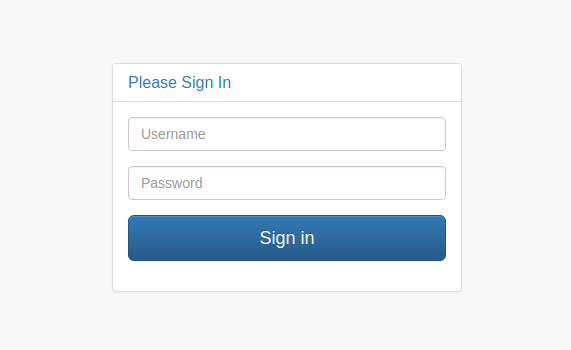
\includegraphics[scale=0.5]{../04_Realisierung/images/loginform.png}
\caption{Login Formular}
\end{figure}

\newpage

\subsection{Demo LwM2M-Client}
\subsection{Allgemein}
Wie auch der Server, ist der LwM2M-Client mit der Leshan Library implementiert. 
Raspberry Pi mit einem Arch Linux + Java Umgebung.
Temperatursensor und Lichtsensor.
Democlient von Leshan übernommen und angepasst.